\appendix
%\section{A pilot experiment with human evaluation}
%\label{sec:appendix}

%We did a pilot experiment on the SAMSum dataset by with vanilla fine-tuned BART. By switching names, we collect two generations for each sample and names are changed back for comparisons. Among the 71.92\% samples with different pairs of outputs, we randomly sampled 200 pairs and asked two human annotators to label each case among 4 choices mentioned in Sec.5.5. 

%According to the results in Table~\ref{tab:pilot}, the inter-annotator agreement is almost perfect and the most severe unfairness is from content distinction. This inspired us to design the following loss function.

%\begin{table}[h]
%	\scriptsize
%	\centering
%	\begin{tabular}{crrrrr}
	%	\hline
%		\textbf{Annotator} & \textbf{Cont} &\textbf{Spea} & \textbf{Reas}  & \textbf{Expre} & \textbf{Kappa} \\
%		\hline
%		1 & 64.50 & 3.00 & 11.00 & 21.50 & \multirow{2}{*}{95.94}\\
%		2 & 64.50 & 3.00 & 13.00 & 19.50 & \\
		
%		\hline
%	\end{tabular}
%	\caption{The percentage of different labels(\%) and Kappa score(\%) between two annotators.}
%	\label{tab:pilot}
%\end{table}



\section{Illustration for Insensitivity Losses}
\label{sec:app-model}

Fig.~\ref{fig:model} depicts the positions of the cross attentions and the final decoder hidden states in the encoder-decoder Transformer model for a better understanding of our two insensitivity losses.

\begin{figure*}[]
	\centering
	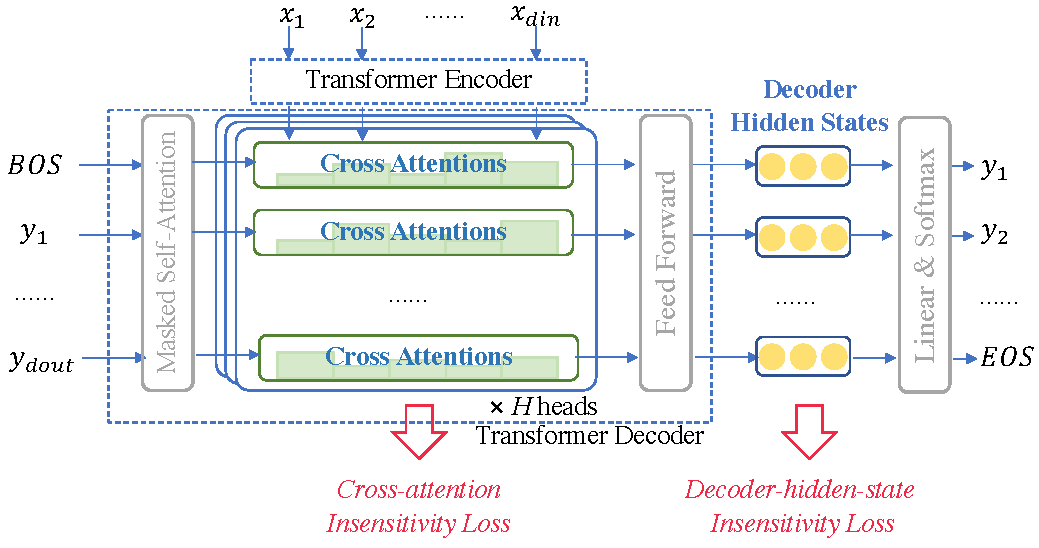
\includegraphics[scale=0.6]{model.pdf}
	\caption{An illustration of insensitive losses. BOS and EOS are special tokens standing for the start and the end of the output.} %in the summaries.}
	%\underline{Divergent contents} are underlined in the generated summaries.}
	\label{fig:model}
\end{figure*}

\section{Name Groups}
\label{sec:app-names}
To collect polysemous, rare and unknown names, we counted the number of occurrences of all-possible names in the pre-training corpus, Wikipedia\footnote{{https://huggingface.co/datasets/wikipedia}} and BookCorpus\footnote{https://huggingface.co/datasets/bookcorpus}. We denote the frequency of a name as $f_{exact}$ and $f_{ner}$ representing doing exact string match or named entity recognition when counting name occurrences respectively. Rare contains names shown at least once and with the lowest $f_{exact}$ not equaling 0. Unknown includes names with $f_{exact}$ equaling 0. According to our observations, we find that names with a larger $f_{exact}$ are likely to be polysemy and are not uniquely used as personal names. 
So, we design a metric to recognize such names as follows:
\begin{equation}
	u = \frac{rank(f_{exact})-rank(f_{ner})}{rank(f_{exact})+rank(f_{ner})}
	\label{eq:uniqueness}
\end{equation}
$rank(\cdot)$ means that the ranking of a name among the whole name list based on its frequency in descending order~\footnote{Doing named entity recognition on the whole pre-training corpus is too time-consuming. Therefore, we randomly sample 1\% of the data for counting the $f_{ner}$ and use the name rankings in Eq.~\ref{eq:uniqueness} to get the uniqueness score}. A higher $u$ shows a higher level of uniqueness of a word as a name. The names with the lowest $u$ scores are selected as Polysemous in Sec.~\ref{sec:unfairness}.

Examples of names in different name groups are listed as follows:
\begin{itemize}
	\item \textbf{Frequent}: Alexis, Philip, Matthew, Frank, Tyler, Roy, Catherine, Joan, Amanda, Henry
	\item \textbf{Polysemous}: July, Sea, March, Paris, Treasure, Oxford, Romania, Ice, Jersey, Navy
	\item \textbf{Rare}: Makinzy, Diyanna, Javione, Zamire, Harkeem, Jerralyn, Crissi, Monque, Ajahar, Dijion
	\item \textbf{Unknown}: Jaliyiah, Cardelia, Ravindr, Josephanthony, Tyjohn, Tnaya, Jyren, Kashaunda, Jaykob, Latonnia
	\item \textbf{White}: Kim, Georgia, Joseph, Mark, Martin, James, William, Barbara, Richard, Victoria
	\item \textbf{Hispanic}: Sofia, Daisy, Luis, Manuel, Dora, Emilia, Minerva, Antonio, Oscar, Francisco
	\item \textbf{Black}: Kenya, Ebony, Anderson, Kelvin, Dexter, Cleveland, Percy, Mamie, Jarvis, Essie
	\item \textbf{Asian}: Kong, Muhammad, Gang, Mai, Chi, Krishna, Can, Wan, Wang, Ferdinand
\end{itemize}





\section{Hyper-parameter Search}
\label{sec:app-hyper}
We empirically searched the hyper-parameters $\alpha$ and $\beta$ in \{1, 10, 20\} respectively with 9 combinations for Ins. Due to the limited computation resources and the large search space, we trained the model with different combinations for a single time, selected the best 3 combinations and 
repeated experiments with different random seeds to determine the final choice of $\alpha$ and $\beta$ according to the performance on $D_{va}$. Finally, we set ($\alpha$, $\beta$) as (1, 10), (1, 10), (1,1) for dialogue summarization, question generation and reading comprehension respectively. We directly borrow these settings for FreIns.

In Fig.~\ref{fig:hyper}, we show the performances of Ins under different combinations for dialogue summarization on the vanilla test set with a single run. We can see that all of the results outperform the baselines in Table~\ref{tab:mdresults-vanilla} and the standard deviation of BertScore among different combinations is only 0.14\%, showing the stable improvements of Ins over the baselines.

\begin{figure}[t]
	\centering
	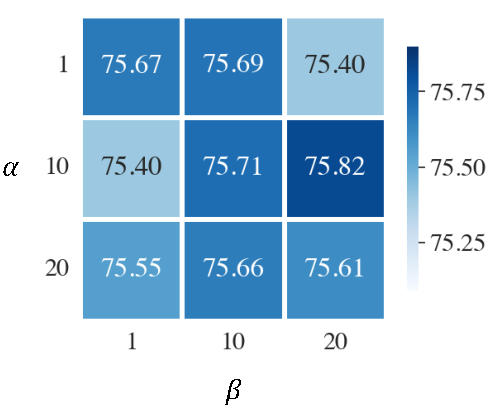
\includegraphics[scale=0.6]{hyper-parameters.pdf}
	\caption{BertScore(\%) on the vanilla test set with different hyper-parameters.} %in the summaries.}
	%\underline{Divergent contents} are underlined in the generated summaries.}
	\label{fig:hyper}
\end{figure}



\section{Additional Results of Sensitivity on an Individual Speaker}
\label{sec:app-results}
Results for sensitivity on an individual speaker on all of the three tasks are in Table~\ref{tab:speaker-off} and Table~\ref{tab:speaker-on}. Both tables lead to the same observations and conclusions as discussed in Sec~\ref{sec:mda} and Sec~\ref{sec:onlineapproach}, where Ins and FreIns perform best among offline and online approaches correspondingly. 

\begin{table}[h!]
	\scriptsize
	\centering
	\begin{subtable}{\linewidth}
		\scriptsize
		\centering
		\begin{tabular}{p{0.9cm}|p{0.36cm}p{0.36cm}p{0.36cm}p{0.36cm}|p{0.36cm}p{0.36cm}p{0.36cm}p{0.38cm}}
			\toprule[1pt]
			
			& \multicolumn{4}{c|}{\textbf{R2}} & \multicolumn{4}{c}{\textbf{BertScore}} \\
			%\cline{2-9}
			\textbf{Approach}& - & S$\downarrow$ & R$\downarrow$ & D$\downarrow$ & - & S$\downarrow$  & R$\downarrow$ & D$\downarrow$\\
			%& \multicolumn{6}{c}{\textbf{Change-one-name}} \\
			%\textbf{Approach} & \textbf{R2} & \textbf{BertS} & \textbf{D-R2} & \textbf{R-R2} & \textbf{D-BertS} & \textbf{R-BertS} \\
			
			\hline
			\multicolumn{7}{l}{\textit{In-distribution Names}}\\
			Vanilla &
			27.29 & 25.53 & 11.05& 4.42& 74.64&9.65&5.19 & 2.05\\
			Emb & 27.41 & 24.20  & 10.87 & 4.33&74.90&9.49& 5.29& 2.09  \\
			Aug&
			{27.51} &22.24   & {9.89} & {3.96}&74.83&8.50& 4.67& {1.85}  \\
			Ins$\star$  & \textbf{28.70} &\textbf{16.64}& \textbf{7.19} & \textbf{2.92} & \textbf{75.44} &\textbf{6.11} & \textbf{3.18} & \textbf{1.28}\\

			
			\hline
			\multicolumn{7}{l}{\textit{All-possible Names}}\\
			Vanilla &
			27.32&25.77  & 11.07 & 4.45&74.81 &9.61&5.15& 2.04  \\
			Emb & 27.26 & 24,98  & 10.68 & 4.25&74.80&9.57 & 5.16& 2.02\\
			Aug  &
			27.36 & 22.73 & {10.04} & {4.03} &74.86&8.56& 4.69& 1.87  \\
			Ins$\star$ & \textbf{28.38} &\textbf{18.65} & \textbf{8.12}& \textbf{3.29}  &\textbf{75.35} &\textbf{6.89}& \textbf{3.75} & \textbf{1.50} \\

			\bottomrule[1pt]
		\end{tabular}
		\caption{Dialogue Summarization}
		%\label{tab:mdresults-ds}
	\end{subtable}
	
	\begin{subtable}{\linewidth}
		\scriptsize
		\centering
		\begin{tabular}{p{0.9cm}|p{0.36cm}p{0.36cm}p{0.36cm}p{0.36cm}|p{0.36cm}p{0.36cm}p{0.36cm}p{0.36cm}}
			\toprule[1pt]
			 & \multicolumn{4}{c|}{\textbf{BLEU}} & \multicolumn{4}{c}{\textbf{RL}} \\
			%\cline{2-9}
			\textbf{Approach}& - & S$\downarrow$  & R$\downarrow$ & D$\downarrow$& - & S$\downarrow$  & R$\downarrow$& D$\downarrow$ \\
			%& \multicolumn{6}{c}{\textbf{Change-one-name}} \\
			%\textbf{Approach}  & \textbf{Bleu} & \textbf{RL} & \textbf{D-Bleu} & \textbf{R-Bleu} & \textbf{D-RL} & \textbf{R-RL} \\
			
			\hline
			\multicolumn{7}{l}{\textit{In-distribution Names}}\\
			Vanilla &
			17.93& 18.76& 6.08& 2.58&{56.85} &8.17&7.55& 3.12 \\
			Emb  & 18.34 &22.22 & 7.63 & 3.26 &56.84 & 10.07 & 9.62 & 3.98\\
			Aug &
			18.06 & 14.82 & {4.39} & {1.90} &56.12 &6.91 & {6.38} & 2.69 \\
			Ins$\star$ & \textbf{19.45} &\textbf{9.66}  & \textbf{2.75} & \textbf{1.18}& \textbf{57.31}&\textbf{4.50}& \textbf{4.27} & \textbf{1.81} \\
			%Ins+ & 18.78 & 56.97 & 3.08 & 7.21 & 4.01 & 9.73 &\\
			
			\hline
			\multicolumn{7}{l}{\textit{All-possible Names}}\\
			Vanilla &
			17.91& 17.73& 5.75 & 2.46&56.67 & 7.76&7.05 & 2.95\\
			Emb  & 18.67 & 20.80  & 7.08& 3.06&56.86& 9.47& 8.89 & 3.73 \\
			Aug  &
			17.97 & 13.04 & {3.62} & {1.57} &56.12&6.06& {6.50}& {2.25}  \\
			Ins$\star$& \textbf{19.60} & \textbf{8.11} & \textbf{2.22} & \textbf{0.97}& \textbf{57.51}&\textbf{3.77}& \textbf{3.42}& \textbf{1.47} \\

			\bottomrule[1pt]
		\end{tabular}
		\caption{Question Generation}
		%\label{tab:mdresults-qg}
	\end{subtable}
	
	\begin{subtable}{\linewidth}
		\scriptsize
		\centering
		\begin{tabular}{p{0.9cm}|p{0.36cm}p{0.36cm}p{0.36cm}p{0.36cm}|p{0.36cm}p{0.36cm}p{0.36cm}p{0.36cm}}
			\toprule[1pt]
			 & \multicolumn{4}{c|}{\textbf{BLEU}} & \multicolumn{4}{c}{\textbf{RL}} \\
			%\cline{2-9}
			\textbf{Approach}& - & S$\downarrow$  & R$\downarrow$ & D$\downarrow$& - & S$\downarrow$ & R$\downarrow$ & D$\downarrow$ \\
			%& \multicolumn{6}{c}{\textbf{Change-one-name}} \\
			%\textbf{Approach}  & \textbf{Bleu} & \textbf{RL} & \textbf{D-Bleu} & \textbf{R-Bleu} & \textbf{D-RL} & \textbf{R-RL} \\
			
			\hline
			\multicolumn{7}{l}{\textit{In-distribution Names}}\\
			Vanilla &
			27.96 &54.08& 3.85 & 1.67 & 73.91 &4.49 & 5.50 & 2.37\\
			Emb & 25.52 & 56.61 & 4.28 & 1.85&70.20& 5.32 & 6.37& 2.75 \\
			Aug  &
			26.54 &  54.76 & 3.69 & 1.60&72.53&4.57& 5.87& 2.55 \\
			Ins$\star$& \textbf{29.03} &\textbf{52.03}  & \textbf{2.48} & \textbf{1.08}& \textbf{74.81}&\textbf{5.65}& \textbf{4.41}& \textbf{1.91}  \\
			%Ins+ & 18.78 & 56.97 & 3.08 & 7.21 & 4.01 & 9.73 &\\
			
			\hline
			\multicolumn{7}{l}{\textit{All-possible Names}}\\
			Vanilla&
			27.82 &53.48 & 2.81 & 1.22 &73.97 & 3.28& 4.07& 1.77 \\
			Emb & 25.14 & 56.08 & 3.04 & 1.32 &70.51&4.31& 4.89 & 2.12 \\
			Aug &
			26.64 &  53.71 & 2.92& 1.27 &72.68&3.61& 4.61& 2.00  \\
			Ins$\star$  & \textbf{29.40} & \textbf{51.20}& \textbf{1.93} & \textbf{0.83} & \textbf{74.94}&\textbf{2.41} & \textbf{3.13}& \textbf{1.36} \\
			%Ins+ & 18.78 & 57.07 & 2.61 & 6.09 & 3.46 & 8.24 &\\
			\bottomrule[1pt]
		\end{tabular}
		\caption{Reading Comprehension}
		%\label{tab:mdresults-rc}
	\end{subtable}
	\caption{Performances(\%) of offline approaches for sensitivity on an individual speaker.}	
	\label{tab:speaker-off}
\end{table}




\begin{table}[h!]
	\scriptsize
	\centering
	\begin{subtable}{\linewidth}
		\scriptsize
		\centering
		\begin{tabular}{p{0.9cm}|p{0.36cm}p{0.36cm}p{0.36cm}p{0.36cm}|p{0.36cm}p{0.36cm}p{0.36cm}p{0.38cm}}
			\toprule[1pt]
			
			 & \multicolumn{4}{c|}{\textbf{R2}} & \multicolumn{4}{c}{\textbf{BertScore}} \\
			%\cline{2-9}
			\textbf{Approach}& - & S$\downarrow$ & R$\downarrow$ & D$\downarrow$ & - & S$\downarrow$  & R$\downarrow$ & D$\downarrow$\\
			%& \multicolumn{6}{c}{\textbf{Change-one-name}} \\
			%\textbf{Approach}  & \textbf{R2} & \textbf{BertS} & \textbf{D-R2} & \textbf{R-R2} & \textbf{D-BertS} & \textbf{R-BertS} \\
			
			\hline
			%Vanilla & 28.12 & 75.09 & - &-&-&-&-&-&-&-&-&-\\
			%ID &-&-&-&-&-&-&-&\\
			Fre  &
			{28.40} &20.28 & 9.25 & 3.73 &75.10 &7.85& 4.29& 1.72  \\
			FreAug  &
			27.91 &  20.11 & {9.02}& {3.64}&{74.97}&7.78& 4.24 & 1.70 \\
			FreIns$\star$ & \textbf{28.58} &\textbf{13.29 }  & \textbf{5.99}& \textbf{2.46} &\textbf{75.42}&\textbf{4.91} & \textbf{2.68} & \textbf{1.09}\\
			\bottomrule[1pt]
		\end{tabular}
		\caption{Dialogue Summarization}
		%\label{tab:ddresults-ds}
	\end{subtable}
	
		\begin{subtable}{\linewidth}
		\scriptsize
		\centering
		\begin{tabular}{p{0.9cm}|p{0.36cm}p{0.36cm}p{0.36cm}p{0.36cm}|p{0.36cm}p{0.36cm}p{0.36cm}p{0.36cm}}
			\toprule[1pt]
			 & \multicolumn{4}{c|}{\textbf{BLEU}} & \multicolumn{4}{c}{\textbf{RL}} \\
		%	\cline{2-9}
			\textbf{Approach}& - & S$\downarrow$ & R$\downarrow$ & D$\downarrow$ & - & S$\downarrow$  & R$\downarrow$& D$\downarrow$ \\
			%& \multicolumn{6}{c|}{\textbf{Change-all-name}} & \multicolumn{6}{c}{\textbf{Change-one-name}} \\
			%\textbf{Approach} & \textbf{Bleu} & \textbf{RL} & \textbf{D-Bleu} & \textbf{R-Bleu} & \textbf{D-RL} & \textbf{R-RL} \\
			
			\hline
			%Vanilla & 18.57 & 56.40 & - &-&-&-&-&-&-&-&-&-\\
			%ID &-&-&-&-&-&-\\
			Fre &
			{18.90} &10.59& 2.97 & 1.29 & 57.01 & 4.76& 4.09 & 1.74\\
			FreAug  &
			18.60 & 8.62 & 2.54 & 1.10 &{57.13}&3.81& 3.46& 1.48  \\
			FreIns$\star$  & \textbf{19.29} & \textbf{5.48}  & \textbf{1.76}& \textbf{0.77} &\textbf{56.91}&\textbf{2.39} & \textbf{2.18}& \textbf{0.94}\\
			\bottomrule[1pt]
		\end{tabular}
		\caption{Question Generation}
		%\label{tab:ddresults-qg}
	\end{subtable}

	\begin{subtable}{\linewidth}
		\scriptsize
		\centering
		\begin{tabular}{p{0.9cm}|p{0.36cm}p{0.36cm}p{0.36cm}p{0.36cm}|p{0.36cm}p{0.36cm}p{0.36cm}p{0.36cm}}
			\toprule[1pt]
			 & \multicolumn{4}{c|}{\textbf{BLEU}} & \multicolumn{4}{c}{\textbf{RL}} \\
			%\cline{2-9}
			\textbf{Approach}& - & S$\downarrow$ & R$\downarrow$ & D$\downarrow$ & - & S$\downarrow$ & R$\downarrow$ & D$\downarrow$ \\
			%& \multicolumn{6}{c|}{\textbf{Change-all-name}} & \multicolumn{6}{c}{\textbf{Change-one-name}} \\
			%\textbf{Approach} & \textbf{Bleu} & \textbf{RL} & \textbf{D-Bleu} & \textbf{R-Bleu} & \textbf{D-RL} & \textbf{R-RL} \\
			
			\hline
			%Vanilla & 28.42 & 73.33 & - &-&-&-&-&-&-&-&-&-\\
			%ID &-&-&-&-&-&-\\
			Fre &
			27.15 & 53.86 & 2.07 & 0.89 &73.89&2.67& 3.22 & 1.39 \\
			FreAug  & 27.82 & \textbf{52.03}& 1.83 & 0.80 &74.32 & 2.33& 3.08 & 1.33\\
			FreIns$\star$ & \textbf{28.57} & 52.41  & \textbf{1.46}& \textbf{0.64} &\textbf{74.89}&\textbf{1.70}& \textbf{2.36}& \textbf{1.02}  \\
			
			\bottomrule[1pt]
			
		\end{tabular}
		\caption{Reading Comprehension}
		%\label{tab:ddresults-rc}
	\end{subtable}


	\caption{Performances(\%) of online approaches for sensitivity on an individual speaker.}	
	\label{tab:speaker-on}
\end{table}


\section{Case study}

We show cases for different tasks in this section.

\begin{figure}[h!]
	\centering
	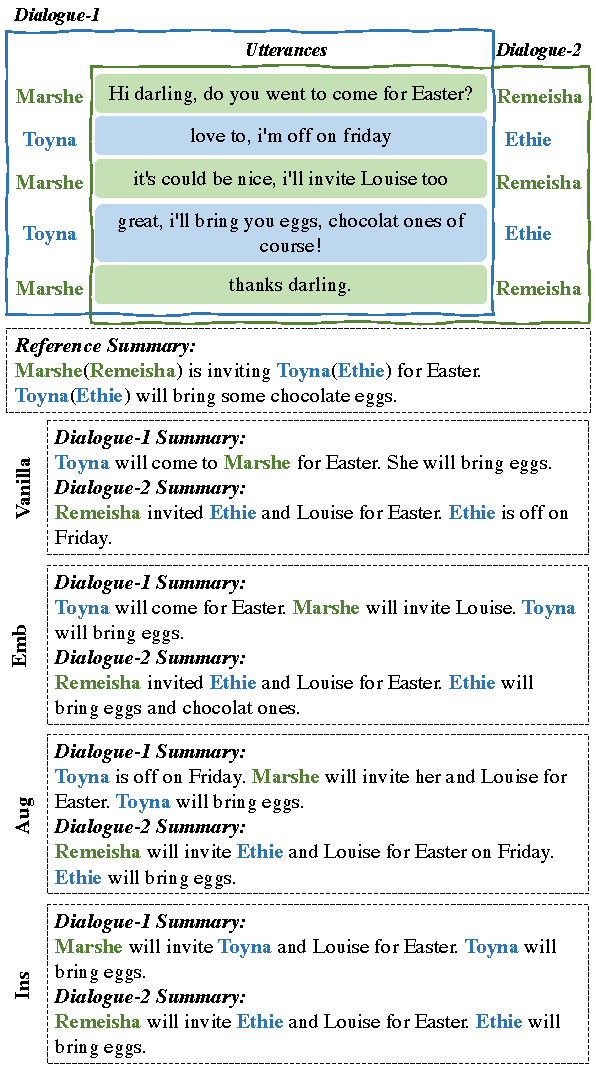
\includegraphics[width=0.95\linewidth]{case-ds.pdf}
	\caption{Case study for dialogue summarization.} 
	\label{fig:case-ds}
\end{figure}

\begin{figure}[t!]
	\centering
	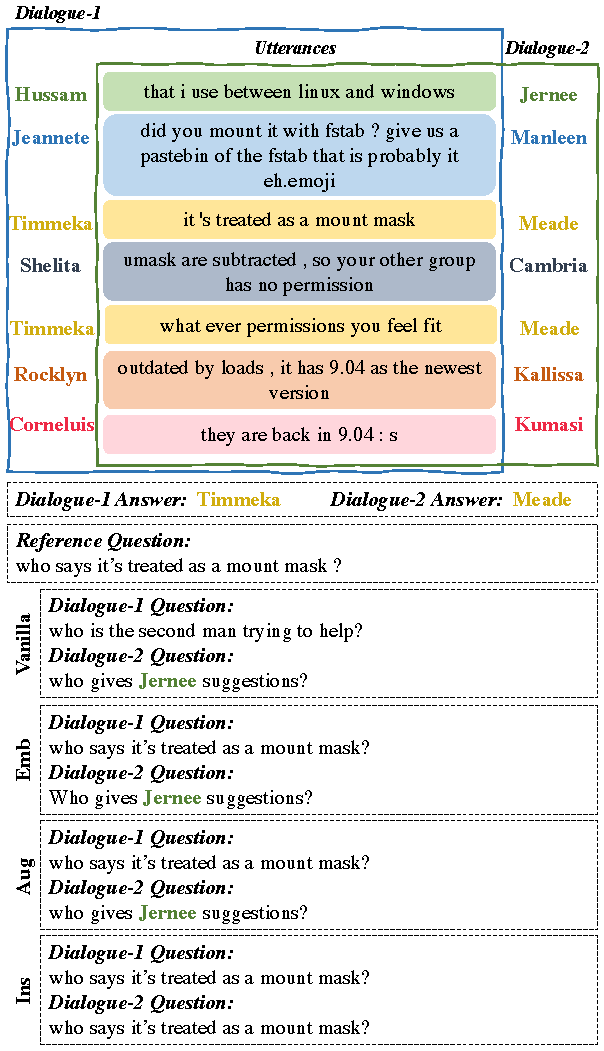
\includegraphics[width=0.95\linewidth]{case-qg.pdf}
	\caption{Case study for question generation.} 
	\label{fig:case-qg}
\end{figure}

\begin{figure}[h]
	\centering
	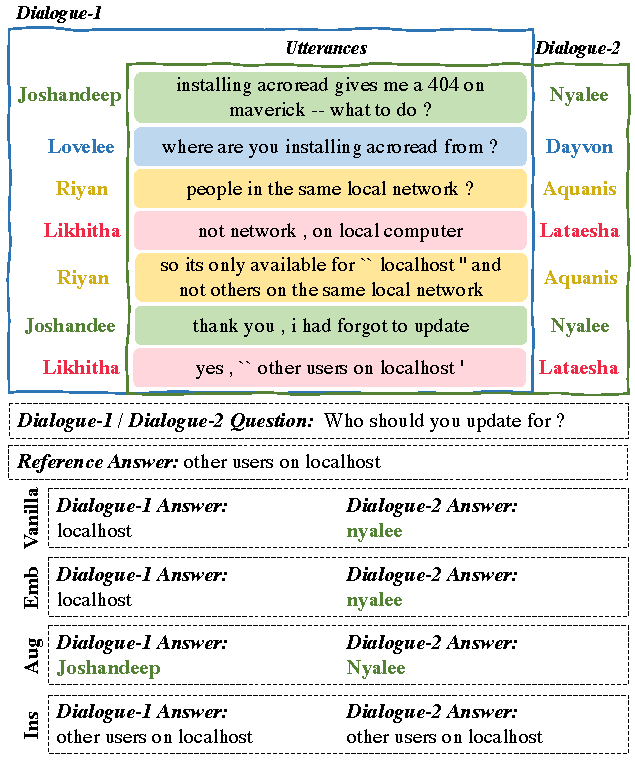
\includegraphics[width=0.95\linewidth]{case-rc.pdf}
	\caption{Case study for reading comprehension.} 
	\label{fig:case-rc}
\end{figure}

The case for dialogue summarization is in Fig.~\ref{fig:case-ds}. Vanilla extracts different information for two sets of names: ``She will bring eggs'' and ``Ethie is off on Friday''. It also uses different expressions: ``will come to ... for Easter'' and ``invited ... for Easter''. Besides, ``Louise'' is only mentioned in the second summary.
Emb has the information difference and the expression difference. Meanwhile, it outputs incorrect content in the second summary, where ``chocolat ones'' is used for describing ``eggs'' in the input dialogue. 
Aug outputs more information for the first set of names. Ins treats the two sets of names equally with the same generations modulo the speaker names.

In the case of question generation in Fig.~\ref{fig:case-qg}, all baselines generate ``who gives Jernee suggestions?'' for the second set of names, which is an inaccurate question with multiple candidate answers. Emb also generates a ``Who'' with the capitalized first letter, which is also different from the other one with lowercase ``who'' if we compare them strictly. Ins generates identical and accurate questions for the same dialogue with different speaker names.


For reading comprehension in Fig.~\ref{fig:case-rc}, both Vanilla and Emb generate quite different answers for two sets of names. Aug generates consistent but wrong answers considering the one-to-one mapping of speaker names. Ins outputs identical correct and complete answers, outperforming the baselines.

%Fig.~\ref{fig:case-ds}, Fig.~\ref{fig:case-qg} and Fig.~\ref{fig:case-rc}.









%\begin{table*}[th!]
%	\scriptsize
%	\centering
%	\begin{subtable}{\linewidth}
%		\scriptsize
%		\centering
%		\begin{tabular}{p{1.2cm}|llllll|llllll}
%			\toprule[1pt]
%			& \multicolumn{6}{c|}{\textbf{Change-all-name}} & \multicolumn{6}{c}{\textbf{Change-one-name}} \\
%			\textbf{Approach} & \textbf{R2} & \textbf{BertS} & \textbf{D-R2} & \textbf{R-R2} & \textbf{D-BertS} & \textbf{R-BertS} & \textbf{R2} & \textbf{BertS} & \textbf{D-R2} & \textbf{R-R2} & \textbf{D-BertS} & \textbf{R-BertS} \\
			
%			\hline
%			\multicolumn{13}{l}{\textit{In-distribution Names}}\\
%			Vanilla & 27.66 & 74.90 & 5.51 & 13.98 & 2.49&6.41&
%			27.29 & 74.64 & 4.42& 11.05& 2.05&5.19 \\
%			Emb & 27.63 & 74.91 & 5.20 & 13.21 & 2.43 & 6.26 & 27.41 & 74.90 & 4.33 & 10.87 & 2.09 & 5.29 \\
%			Aug & 27.82 & 74.95 & {{4.86}} & {{12.33}} & {2.57} & {5.77} &
%			{27.51} & 74.83 & {3.96} & {9.89} & {1.85} & 4.67 \\
%			Ins (our) & \textbf{28.79} & \textbf{75.48} & \textbf{3.82} & \textbf{9.50} & \textbf{1.71} & \textbf{4.32} & \textbf{28.70} & \textbf{75.44} & \textbf{2.92} & \textbf{7.19} & \textbf{1.28} & \textbf{3.18} \\
			%Ins+ & 27.67 & \textbf{75.26} & \textbf{4.85} & \textbf{12.19} & \textbf{2.20} & \textbf{5.61} & \textbf{27.51} & \textbf{75.07}& \textbf{3.92} & \textbf{9.69} & \textbf{1.77} & \textbf{4.44} \\
			
%			\hline
%			\multicolumn{13}{l}{\textit{All-possible Names}}\\
%			Vanilla & 27.19 & 74.83 & 5.72 & 14.64 & 2.60 & 6.66&
%			27.32& 74.81 & 4.45 & 11.07 & 2.04 &5.15 \\
%			Emb & 27.22 & 74.89 & 5.30 & 13.59 & 2.55 & 6.63 & 27.26 & 74.80 & 4.25 & 10.68 & 2.02 & 5.16\\
%			Aug &{{27.50}} & {74.96} & {4.97 }& {12.56} & {2.25} & {5.76} &
%			27.36 & 74.86 & {4.03} & {10.04} & 1.87 & 4.69 \\
%			Ins (our) &  \textbf{28.44} & \textbf{75.38} & \textbf{4.62} & \textbf{11.58} & \textbf{2.05} & \textbf{5.22} & \textbf{28.38} & \textbf{75.35} & \textbf{3.29} & \textbf{8.12} & \textbf{1.50} & \textbf{3.75} \\

%			\bottomrule[1pt]
%		\end{tabular}
%		\caption{Dialogue Summarization}
%		\label{tab:mdresults-ds}
%	\end{subtable}
	
%	\begin{subtable}{\linewidth}
%		\scriptsize
%		\centering
%		\begin{tabular}{p{1.2cm}|llllll|llllll}
%			\toprule[1pt]
%			& \multicolumn{6}{c|}{\textbf{Change-all-name}} & \multicolumn{6}{c}{\textbf{Change-one-name}} \\
%			\textbf{Approach} & \textbf{Bleu} & \textbf{RL} & \textbf{D-Bleu} & \textbf{R-Bleu} & \textbf{D-RL} & \textbf{R-RL} & \textbf{Bleu} & \textbf{RL} & \textbf{D-Bleu} & \textbf{R-Bleu} & \textbf{D-RL} & \textbf{R-RL} \\
			
%			\hline
%			\multicolumn{13}{l}{\textit{In-distribution Names}}\\
%			Vanilla & 18.48 & {57.14} & 5.06 & 11.96 & 5.74&14.19&
%			17.93& {56.85} & 2.58& 6.08& 3.12&7.55 \\
%			Emb & 19.00 & 57.31 & 5.79 & 13.76 & 6.82 & 16.85 & 18.34 & 56.84 & 3.26 & 7.63 & 3.98 & 9.62 \\
%			Aug & 17.89 & 56.26 & {3.52} & {8.22} & {4.69} & {11.35} &
%			18.06 & 56.12 & {1.90} & {4.39} & 2.69 & {6.38} \\
%			Ins (our)& \textbf{19.58} & \textbf{57.47} & \textbf{2.35} & \textbf{5.53} & \textbf{3.35} & \textbf{8.09} & \textbf{19.45} & \textbf{57.31} & \textbf{1.18} & \textbf{2.75} & \textbf{1.81} & \textbf{4.27} \\

			
%			\hline
%			\multicolumn{13}{l}{\textit{All-possible Names}}\\
%			Vanilla & 18.56 & {57.38} & 4.26 & 10.04 & 4.90 & 11.88&
%			17.91& 56.67 & 2.46& 5.75 & 2.95 &7.05 \\
%			Emb & 18.70 & 57.28 & 5.27 & 12.55 & 6.20 & 15.26 & 18.67 & 56.86 & 3.06 & 7.08 & 3.73 & 8.89 \\
%			Aug & 17.81 & 56.08 & {3.06} & {7.15} & {4.03} & {9.64} &
%			17.97 & 56.12 & {1.57} & {3.62} & {2.25} & {6.50} \\
%			Ins (our) & \textbf{19.57} & \textbf{57.49} & \textbf{1.90} & \textbf{4.41} & \textbf{2.78} & \textbf{6.58} & \textbf{19.60} & \textbf{57.51} & \textbf{0.97} & \textbf{2.22} & \textbf{1.47} & \textbf{3.42}\\

%			\bottomrule[1pt]
%		\end{tabular}
%		\caption{Question Generation}
%		\label{tab:mdresults-qg}
%	\end{subtable}
	
%	\begin{subtable}{\linewidth}
%		\scriptsize
%		\centering
%		\begin{tabular}{p{1.2cm}|llllll|llllll}
%			\toprule[1pt]
%			& \multicolumn{6}{c|}{\textbf{Change-all-name}} & \multicolumn{6}{c}{\textbf{Change-one-name}} \\
%			\textbf{Approach} & \textbf{Bleu} & \textbf{RL} & \textbf{D-Bleu} & \textbf{R-Bleu} & \textbf{D-RL} & \textbf{R-RL} & \textbf{Bleu} & \textbf{RL} & \textbf{D-Bleu} & \textbf{R-Bleu} & \textbf{D-RL} & \textbf{R-RL} \\
			
%			\hline
%			\multicolumn{13}{l}{\textit{In-distribution Names}}\\
%			Vanilla &28.34 &73.07 & 2.83 & 6.54 & 4.17 & 9.69 &
%			27.96 & 73.91 & 1.67 & 3.85 & 2.37 & 5.50 \\
	%		Emb & 25.80 & 69.29 & 3.13 & 7.17 & 5.31 & 12.30 & 25.52 & 70.20 & 1.85 & 4.28 & 2.75 & 6.37 \\
%			Aug & 27.07 & 72.11 & 2.62 & 6.04 &  4.50 & 10.42 &
%			26.54 & 72.53 & 1.60 & 3.69 & 2.55 & 5.87\\
%			Ins (our)& \textbf{29.31} & \textbf{74.04} & \textbf{1.97} & \textbf{4.53} & \textbf{3.32} & \textbf{7.66} & \textbf{29.03} & \textbf{74.81} & \textbf{1.08} & \textbf{2.48} & \textbf{1.91} & \textbf{4.41} \\

			
%			\hline
%			\multicolumn{13}{l}{\textit{All-possible Names}}\\
%			Vanilla &  28.56 & 73.60 & 2.34 & 5.39 & 3.53 & 8.21 &
%			27.82 & 73.97 & 1.22 & 2.81 & 1.77 & 4.07 \\
%			Emb & 25.99 & 69.59 & 2.21 & 5.11 & 3.69 & 8.60 & 25.14 & 70.51 & 1.32 & 3.04 & 2.12 & 4.89 \\
%			Aug & 27.12 & 72.23 & 2.23 & 5.15 & 3.58 & 8.29 &
%			26.64 & 72.68 & 1.27 & 2.92 & 2.00 & 4.61 \\
%			Ins (our) & \textbf{29.34} & \textbf{74.35} & \textbf{1.59} & \textbf{3.66} & \textbf{2.64} & \textbf{6.15} & \textbf{29.40} & \textbf{74.94} & \textbf{0.83} & \textbf{1.93} & \textbf{1.36} & \textbf{3.13} \\

%			\bottomrule[1pt]
%		\end{tabular}
%		\caption{Reading Comprehension}
%		\label{tab:mdresults-rc}
%	\end{subtable}
%	\caption{Performances of offline approaches. Scores which are significantly better than Vanilla with p-value$<$0.05 are underlined. $*$ marks the scores whiere p-value of Ins is less than that of Aug.}	
%	\label{tab:mdresults}
%\end{table*}




%\begin{table*}[th!]
%	\scriptsize
%	\centering
%	\begin{subtable}{\linewidth}
%		\scriptsize
%		\centering
%		\begin{tabular}{p{1.2cm}|llllll|llllll}
%			\toprule[1pt]
%			& \multicolumn{6}{c|}{\textbf{Change-all-name}} & \multicolumn{6}{c}{\textbf{Change-one-name}} \\
%			\textbf{Approach} & \textbf{R2} & \textbf{BertS} & \textbf{D-R2} & \textbf{R-R2} & \textbf{D-BertS} & \textbf{R-BertS} & \textbf{R2} & \textbf{BertS} & \textbf{D-R2} & \textbf{R-R2} & \textbf{D-BertS} & \textbf{R-BertS} \\
			
%			\hline
			%Vanilla & 28.12 & 75.09 & - &-&-&-&-&-&-&-&-&-\\
%			ID & 26.97 & 74 26 & - &-&-&-&-&-&-&-&-&-\\
%			Fre & {28.55} & 74.24 & 4.50 & 11.31 & 2.09 & 5.30 &
%			{28.40} & 75.10 & 3.73 & 9.25 & 1.72 & 4.29 \\
%			FreAug & 27.86 & 75.02 & {4.39} & {11.09} & 2.02 & {5.12} &
%			27.91 & {74.97} & {3.64} & {9.02}& 1.70 & 4.24 \\
%			FreIns (our) &  \textbf{28.72} & \textbf{75.53} & \textbf{3.14} & %\textbf{7.66} & \textbf{1.38} & \textbf{3.43} & \textbf{28.58} & \textbf{75.42} & \textbf{2.46} & \textbf{5.99} & \textbf{1.09} & \textbf{2.68} \\
%			\bottomrule[1pt]
%		\end{tabular}
%		\caption{Dialogue Summarization}
%		\label{tab:ddresults-ds}
%	\end{subtable}
	
%	\begin{subtable}{\linewidth}
%		\scriptsize
%		\centering
%		\begin{tabular}{p{1.2cm}|llllll|llllll}
%			\toprule[1pt]
%			& \multicolumn{6}{c|}{\textbf{Change-all-name}} & \multicolumn{6}{c}{\textbf{Change-one-name}} \\
%			\textbf{Approach} & \textbf{Bleu} & \textbf{RL} & \textbf{D-Bleu} & \textbf{R-Bleu} & \textbf{D-RL} & \textbf{R-RL} & \textbf{Bleu} & \textbf{RL} & \textbf{D-Bleu} & \textbf{R-Bleu} & \textbf{D-RL} & \textbf{R-RL} \\
			
%			\hline
			%Vanilla & 18.57 & 56.40 & - &-&-&-&-&-&-&-&-&-\\
%			ID & {19.21} & 56.49 & - &-&-&-&-&-&-&-&-&-\\
%			Fre & {18.96} & {57.10} & 2.35 & 5.51 & 3.04 & 7.23 &
%			{18.90} & 57.01 & 1.29 & 2.97 & 1.74 & 4.09 \\
%			FreAug & 18.52 & 57.06 & 2.14 & 4.92 & 2.76 & 6.50 &
%			18.60 & {57.13} & 1.10 & 2.54 & 1.48 & 3.46 \\
%			FreIns (our) & \textbf{19.71} & \textbf{57.29} & \textbf{1.35} & \textbf{3.12} & \textbf{1.80} & \textbf{4.19} & \textbf{19.29} & \textbf{56.91} & \textbf{0.77} & \textbf{1.76} & \textbf{0.94} & \textbf{2.18}\\
%			\bottomrule[1pt]
%		\end{tabular}
%		\caption{Question Generation}
%		\label{tab:ddresults-qg}
%	\end{subtable}
	
%	\begin{subtable}{\linewidth}
%		\scriptsize
%		\centering
%		\begin{tabular}{p{1.2cm}|llllll|llllll}
%			\toprule[1pt]
%			& \multicolumn{6}{c|}{\textbf{Change-all-name}} & \multicolumn{6}{c}{\textbf{Change-one-name}} \\
%			\textbf{Approach} & \textbf{Bleu} & \textbf{RL} & \textbf{D-Bleu} & \textbf{R-Bleu} & \textbf{D-RL} & \textbf{R-RL} & \textbf{Bleu} & \textbf{RL} & \textbf{D-Bleu} & \textbf{R-Bleu} & \textbf{D-RL} & \textbf{R-RL} \\
			
%			\hline
			%Vanilla & 28.42 & 73.33 & - &-&-&-&-&-&-&-&-&-\\
%			ID & 28.46 & 73.62 & - &-&-&-&-&-&-&-&-&-\\
%			Fre & 27.35 & 73.56 & 1.63 & 3.77 & 2.61 & 6.05 &
%			27.15 & 73.89 & 0.89 & 2.07 & 1.39 & 3.22 \\
%			FreAug & 27.92 & 73.67 & 1.42 & 3.28 & 2.43 & 5.63 & 2.82 & 74.32 & 0.80 & 1.83 & 1.33 & 3.08 \\
%			FreIns (our) &  \textbf{29.03} & \textbf{74.59} & \textbf{1.15} & \textbf{2.66} & \textbf{1.95} & \textbf{4.51} & \textbf{28.57} & \textbf{74.89} & \textbf{0.64} & \textbf{1.46} & \textbf{1.02} & \textbf{2.36} \\
			
%			\bottomrule[1pt]
			
%		\end{tabular}
%		\caption{Reading Comprehension}
%		\label{tab:ddresults-rc}
%	\end{subtable}
	
	
%	\caption{Performances of online approaches on change-all-name test sets. The results on change-all-test sets are in the Appendix. Vanilla is listed for comparisons. Scores which are significantly better than Fre with p-value$<$0.05 are underlined. $*$ marks the scores where p-value of Ins is less than that of FreAug.}	
%	\label{tab:ddresults}
%\end{table*}


%\section{Design Choices of Ins Loss}
